\section{Fahren mit weniger Informationen \dcfirstauthorshort}
\label{ssec:evaluation:messungen:weniger_infos}
Unsere Linienerkennung besteht im wesentlichen aus den zwei fusionierten Komponenten Mittelstrich- und Randlinienerkennung, was die Robustheit unseres Algorithmus wesentlich erhöht. Um zu zeigen, dass diese nicht nur theoretisch unabhängig voneinander funktionieren, wurden zum Test je einmal die Mittellinie und die beiden Randlinien mit weißem Papier verdeckt. 

%Da unser Algorithmus im wesentlichen aus den zwei nahezu unabhängigen, fusionierten Komponenten für die Mittelstrich- und die Randlinienerkennung besteht, soll in diesem Abschnitt gezeigt werden, dass 

\subsection{Fahren ohne Mittellinie}
Da in diesem Test keine Mittellinienpunkte gefunden wurden, konnten die Startpunkte für den Riverflow-Algorithmus nur wie in Kapitel~\ref{sssec:fahrspurerkennung:riverflow:randlinie:startpunktgewinnung} beschrieben mittels der vereinfachten Hough-Transformation oder der Annahme fixer Punkte bestimmt werden. Abbildung~\ref{fig:evaluation:riverflow:ohneMittellinie} zeigt den Versuchsaufbau und das Ergebnis der Karte nach einer erfolgreich gefahrenen Runde ohne Mittellinie.

\begin{figure}[htbp] % [htb]
	%\centering
	%\hfill
	\subfloat[Versuchsaufbau ohne Mittellinie \label{fig:evaluation:riverflow:ohneMittellinie:Versuchsaufbau}]{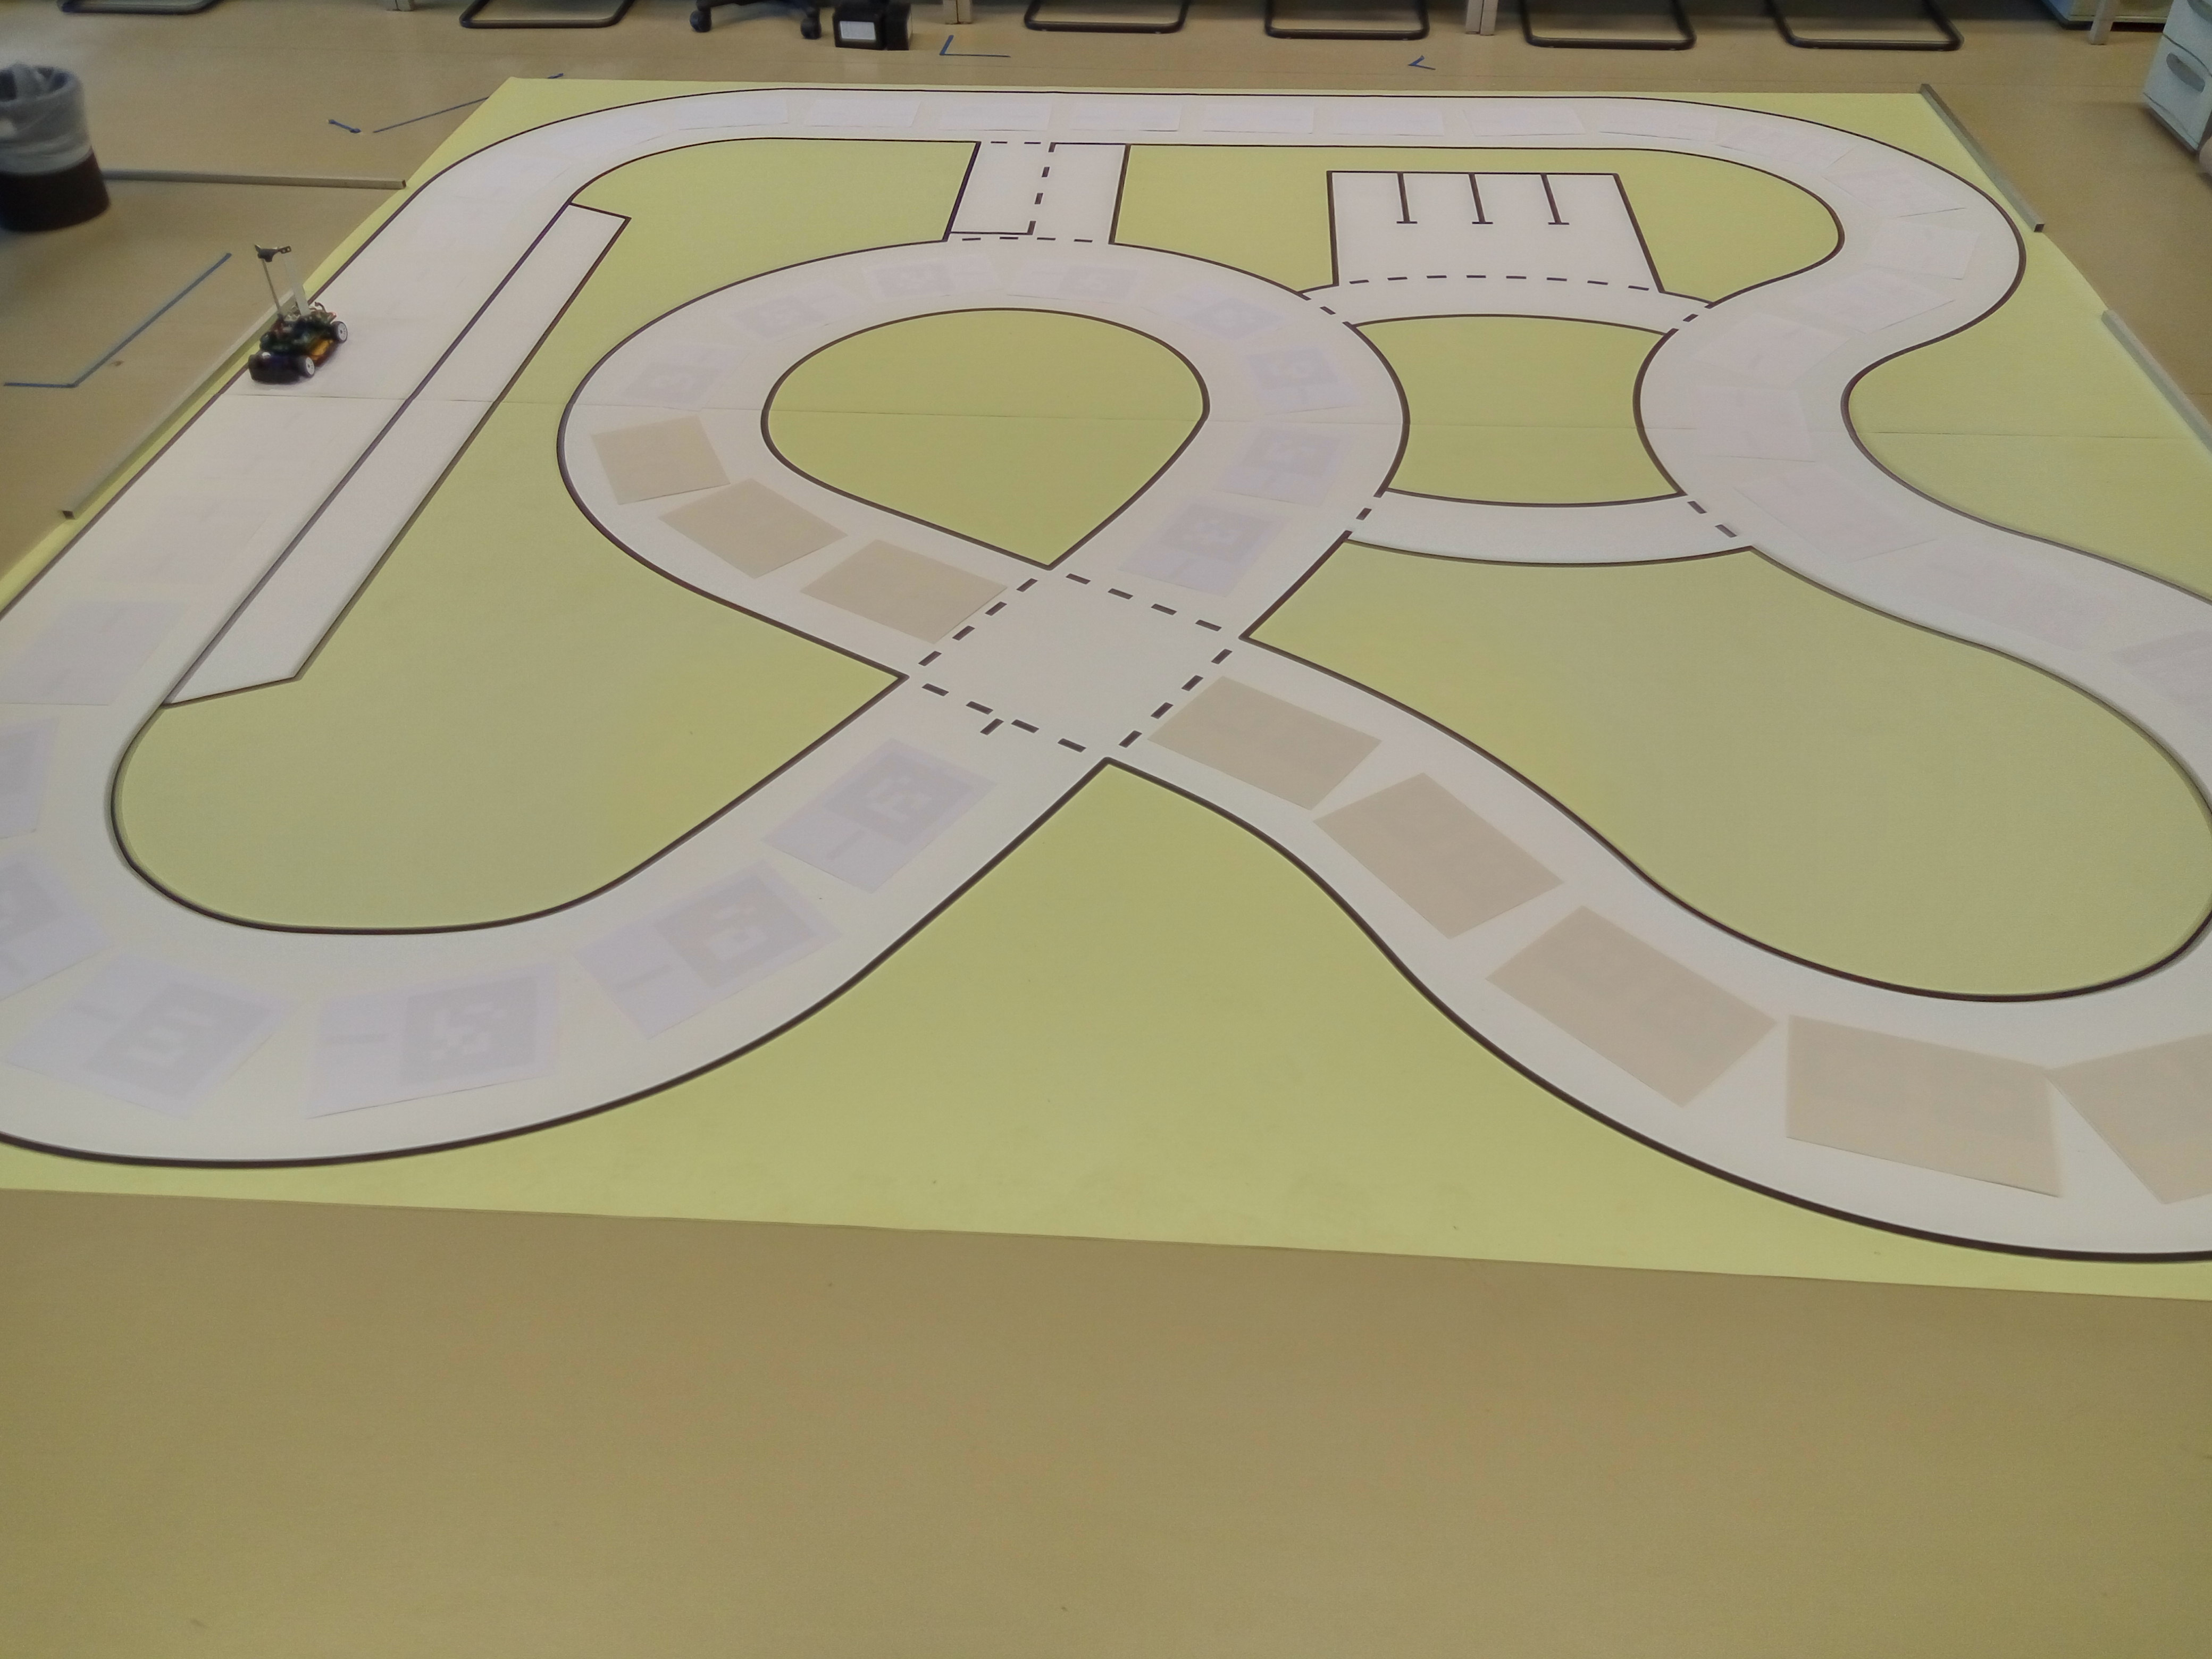
\includegraphics[height=0.28\textheight]{evaluation_riverflow_ohne_mittellinie_versuchsaufbau.jpg}}
	\hfill
	\subfloat[Weltkarte ohne Mittellinie \label{fig:evaluation:riverflow:ohneMittellinie:Weltkarte}]{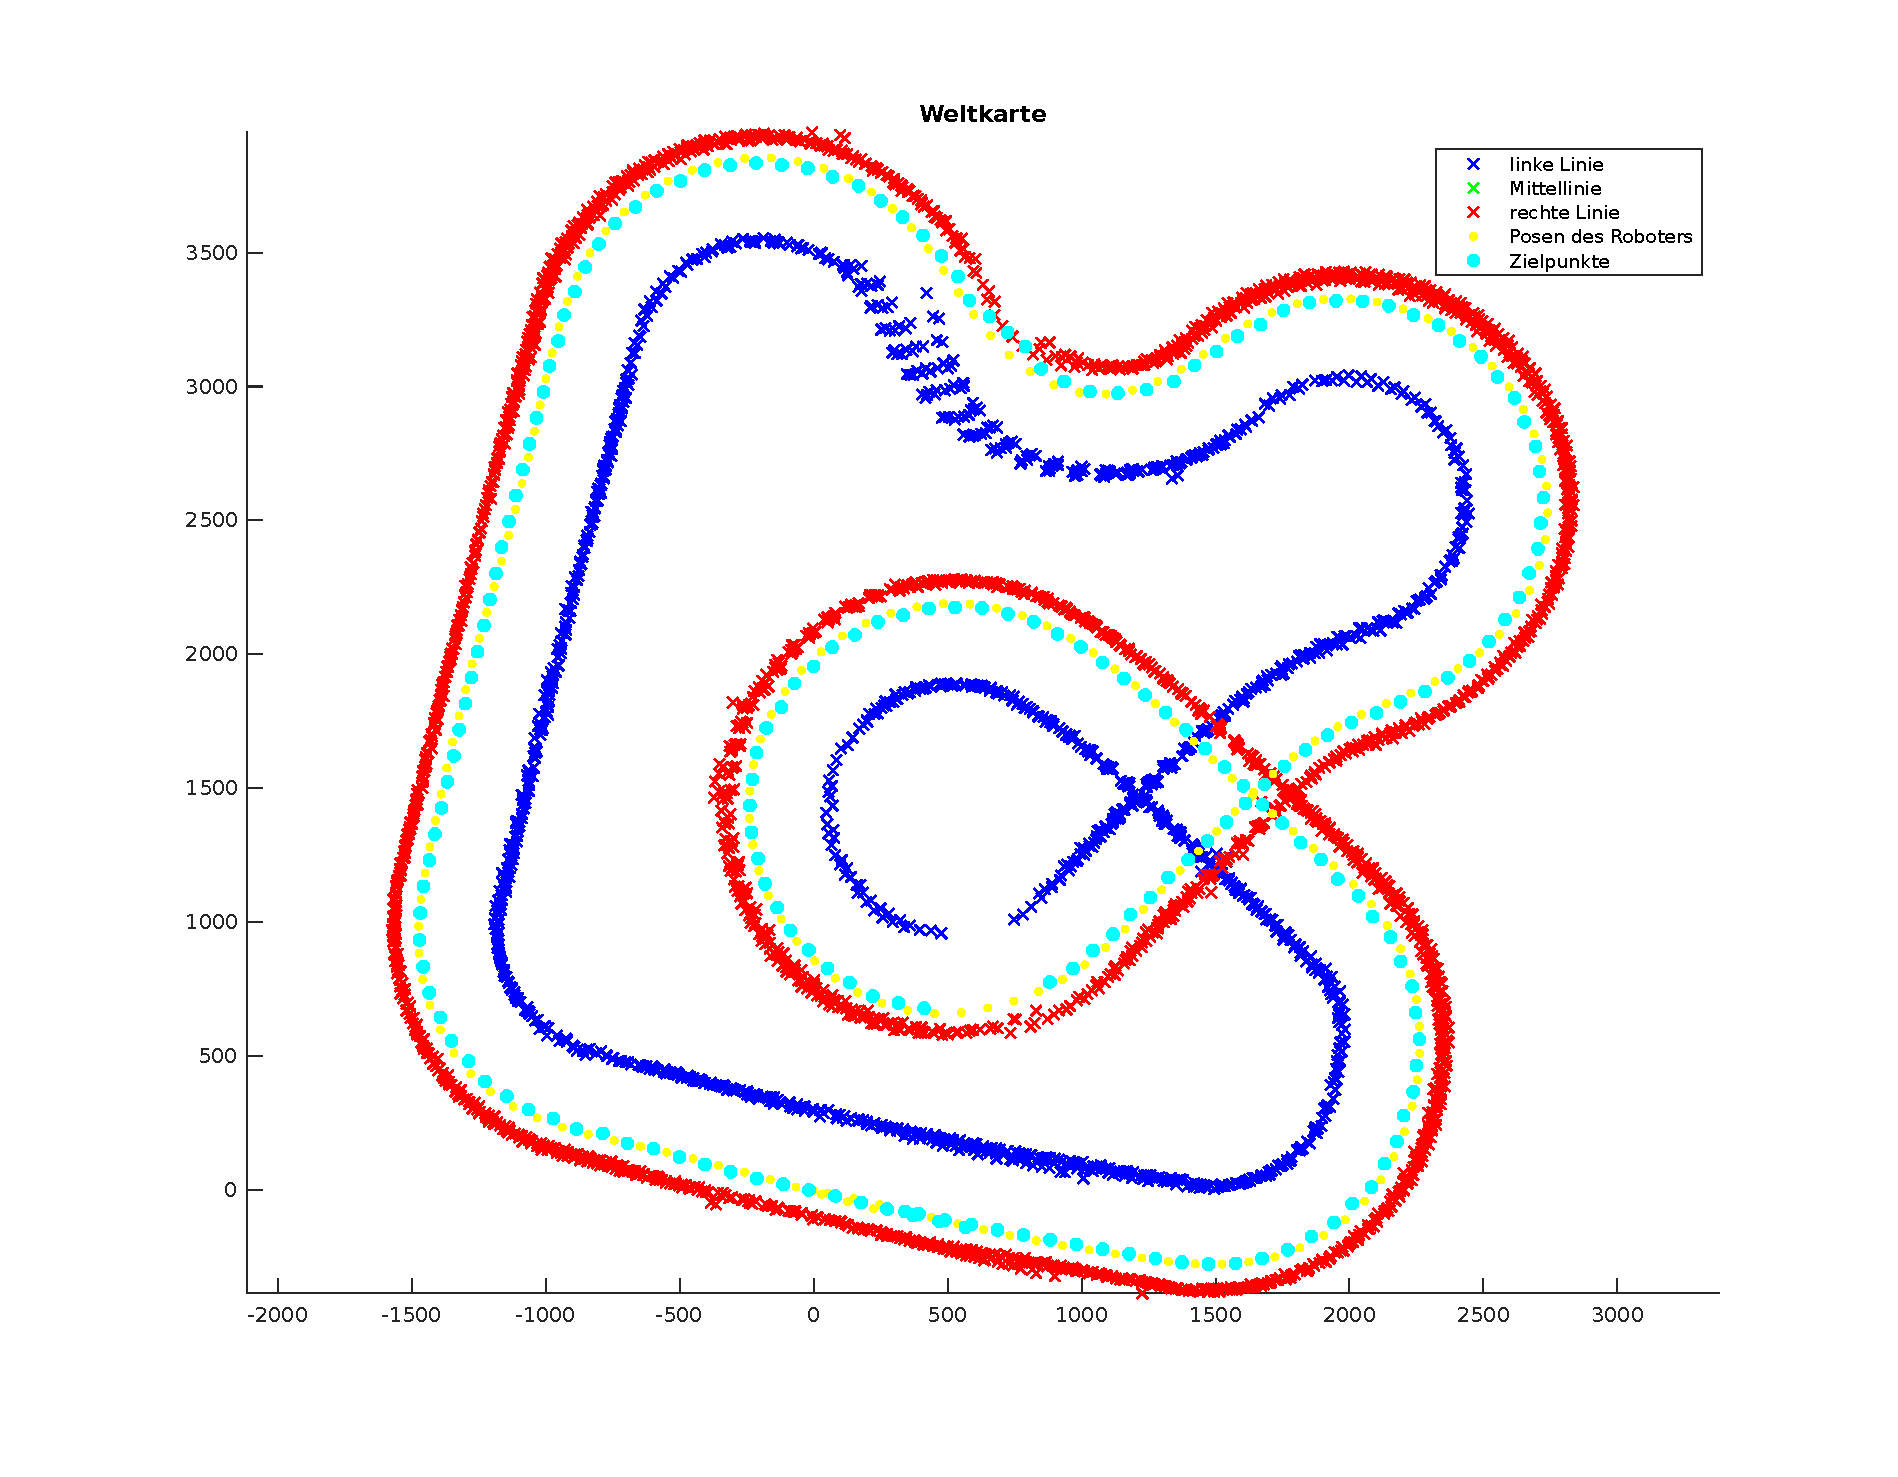
\includegraphics[height=0.28\textheight]{evaluation_riverflow_ohne_mittellinie_worldmap.pdf}}
	\caption{Testfahrt mit durch weißes Papier abgedeckten Mittelstrichen}
	\label{fig:evaluation:riverflow:ohneMittellinie}
\end{figure}

\subparagraph{Probleme}
Damit die gesamte Runde ohne Mittellinie gemeistert werden konnte, wurden während des Versuchs bestimmte Parameter angepasst. Stand der Roboter beispielsweise zu schräg in der Fahrspur, geriet die Randlinie schnell aus dem Bereich, in dem die vereinfachte Hough-Transformation ausgeführt wird. Deshalb wurde die Breite dieses Bildausschnittes vergrößert. 
%, um sich aus höheren Abweichungen des Fahrzeugs von der Fahrspur wieder fangen zu können. 
Dies führt allerdings zu einem Nachteil, welcher der Grund für die anfangs schmalere Einstellung war und in Abbildung~\ref{fig:evaluation:riverflow:ohneMittellinie:problem} dargestellt ist. Da der Hough-Algorithmus nur nach den größten Maxima sucht (siehe Abschnitt~\ref{ssec:grundlagen:hough:vereinfachte}), erkennt er mitunter bei zu breiter Fenstereinstellung benachbarte Markierungen parallel verlaufender Straßen. Die in Kapitel~\ref{ssec:fahrspurerkennung:riverflow:verifikation} erläuterte Verifikation verhindert erfreulicherweise die Aufnahme der falschen Punkte in die Karte. Da der Roboter jedoch auch keine Richtigen erkannte, erhält er in diesem Fall keine neuen Informationen zur Zielpunktfindung. 

Die Startpunktgewinnung mittels Mittellinie bietet darüber hinaus den großen Vorteil, dass die Richtung des Startpunktvektors bekannt ist. Da diese Information hier fehlt, zeigt der Verschiebungsvektor in x-Richtung des Roboterkoordinatensystems. In engen Kurven führt das in ungünstigen Fällen wie in Abbildung~\ref{fig:evaluation:riverflow:ohneMittellinie:problem} zum Abbruch, da die nächste Scanlinie die Fahrbahnmarkierung nicht mehr schneidet. Das ist der Grund für die große Lücke in der linken Linie der in Abbildung~\ref{fig:evaluation:riverflow:ohneMittellinie:Weltkarte} dargestellten Weltkarte. 

\begin{figure}[htbp] % [htb]
	\centering
	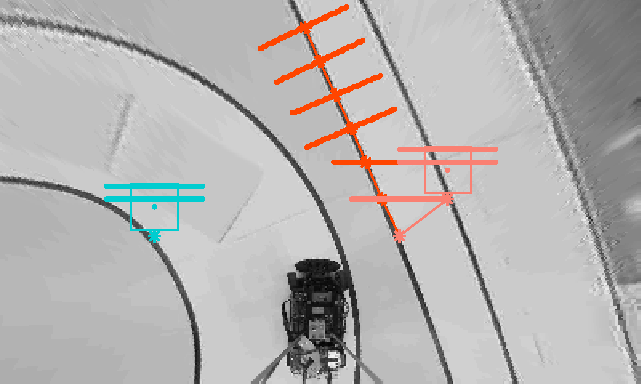
\includegraphics[width=0.7\textwidth]{evaluation_riverflow_ohne_mittellinie_problem_hough.pdf}
	\caption{Ungünstige Position für die mit Hough initialisierte Randlinienerkennung}
	\label{fig:evaluation:riverflow:ohneMittellinie:problem}
\end{figure}

\subsection{Fahren ohne Randlinien}
Die bisher gute Qualität der binarisierten Bilder ermöglicht eine zuverlässige Mittellinienerkennung. Da diese von keinerlei Startpunkten oder Ähnlichem abhängt, stellen auch enge Kurven oder benachbarte Straßenabschnitte kein Problem dar. Der Versuchsaufbau und die zugehörig aufgenommene Weltkarte sind in Abbildung~\ref{fig:evaluation:riverflow:ohneRandlinie} dargestellt.

\begin{figure}[htbp] % [htb]
%	\centering
	%\hfill
	\subfloat[Versuchsaufbau ohne Randlinien \label{fig:evaluation:riverflow:ohneRandlinie:Versuchsaufbau}]{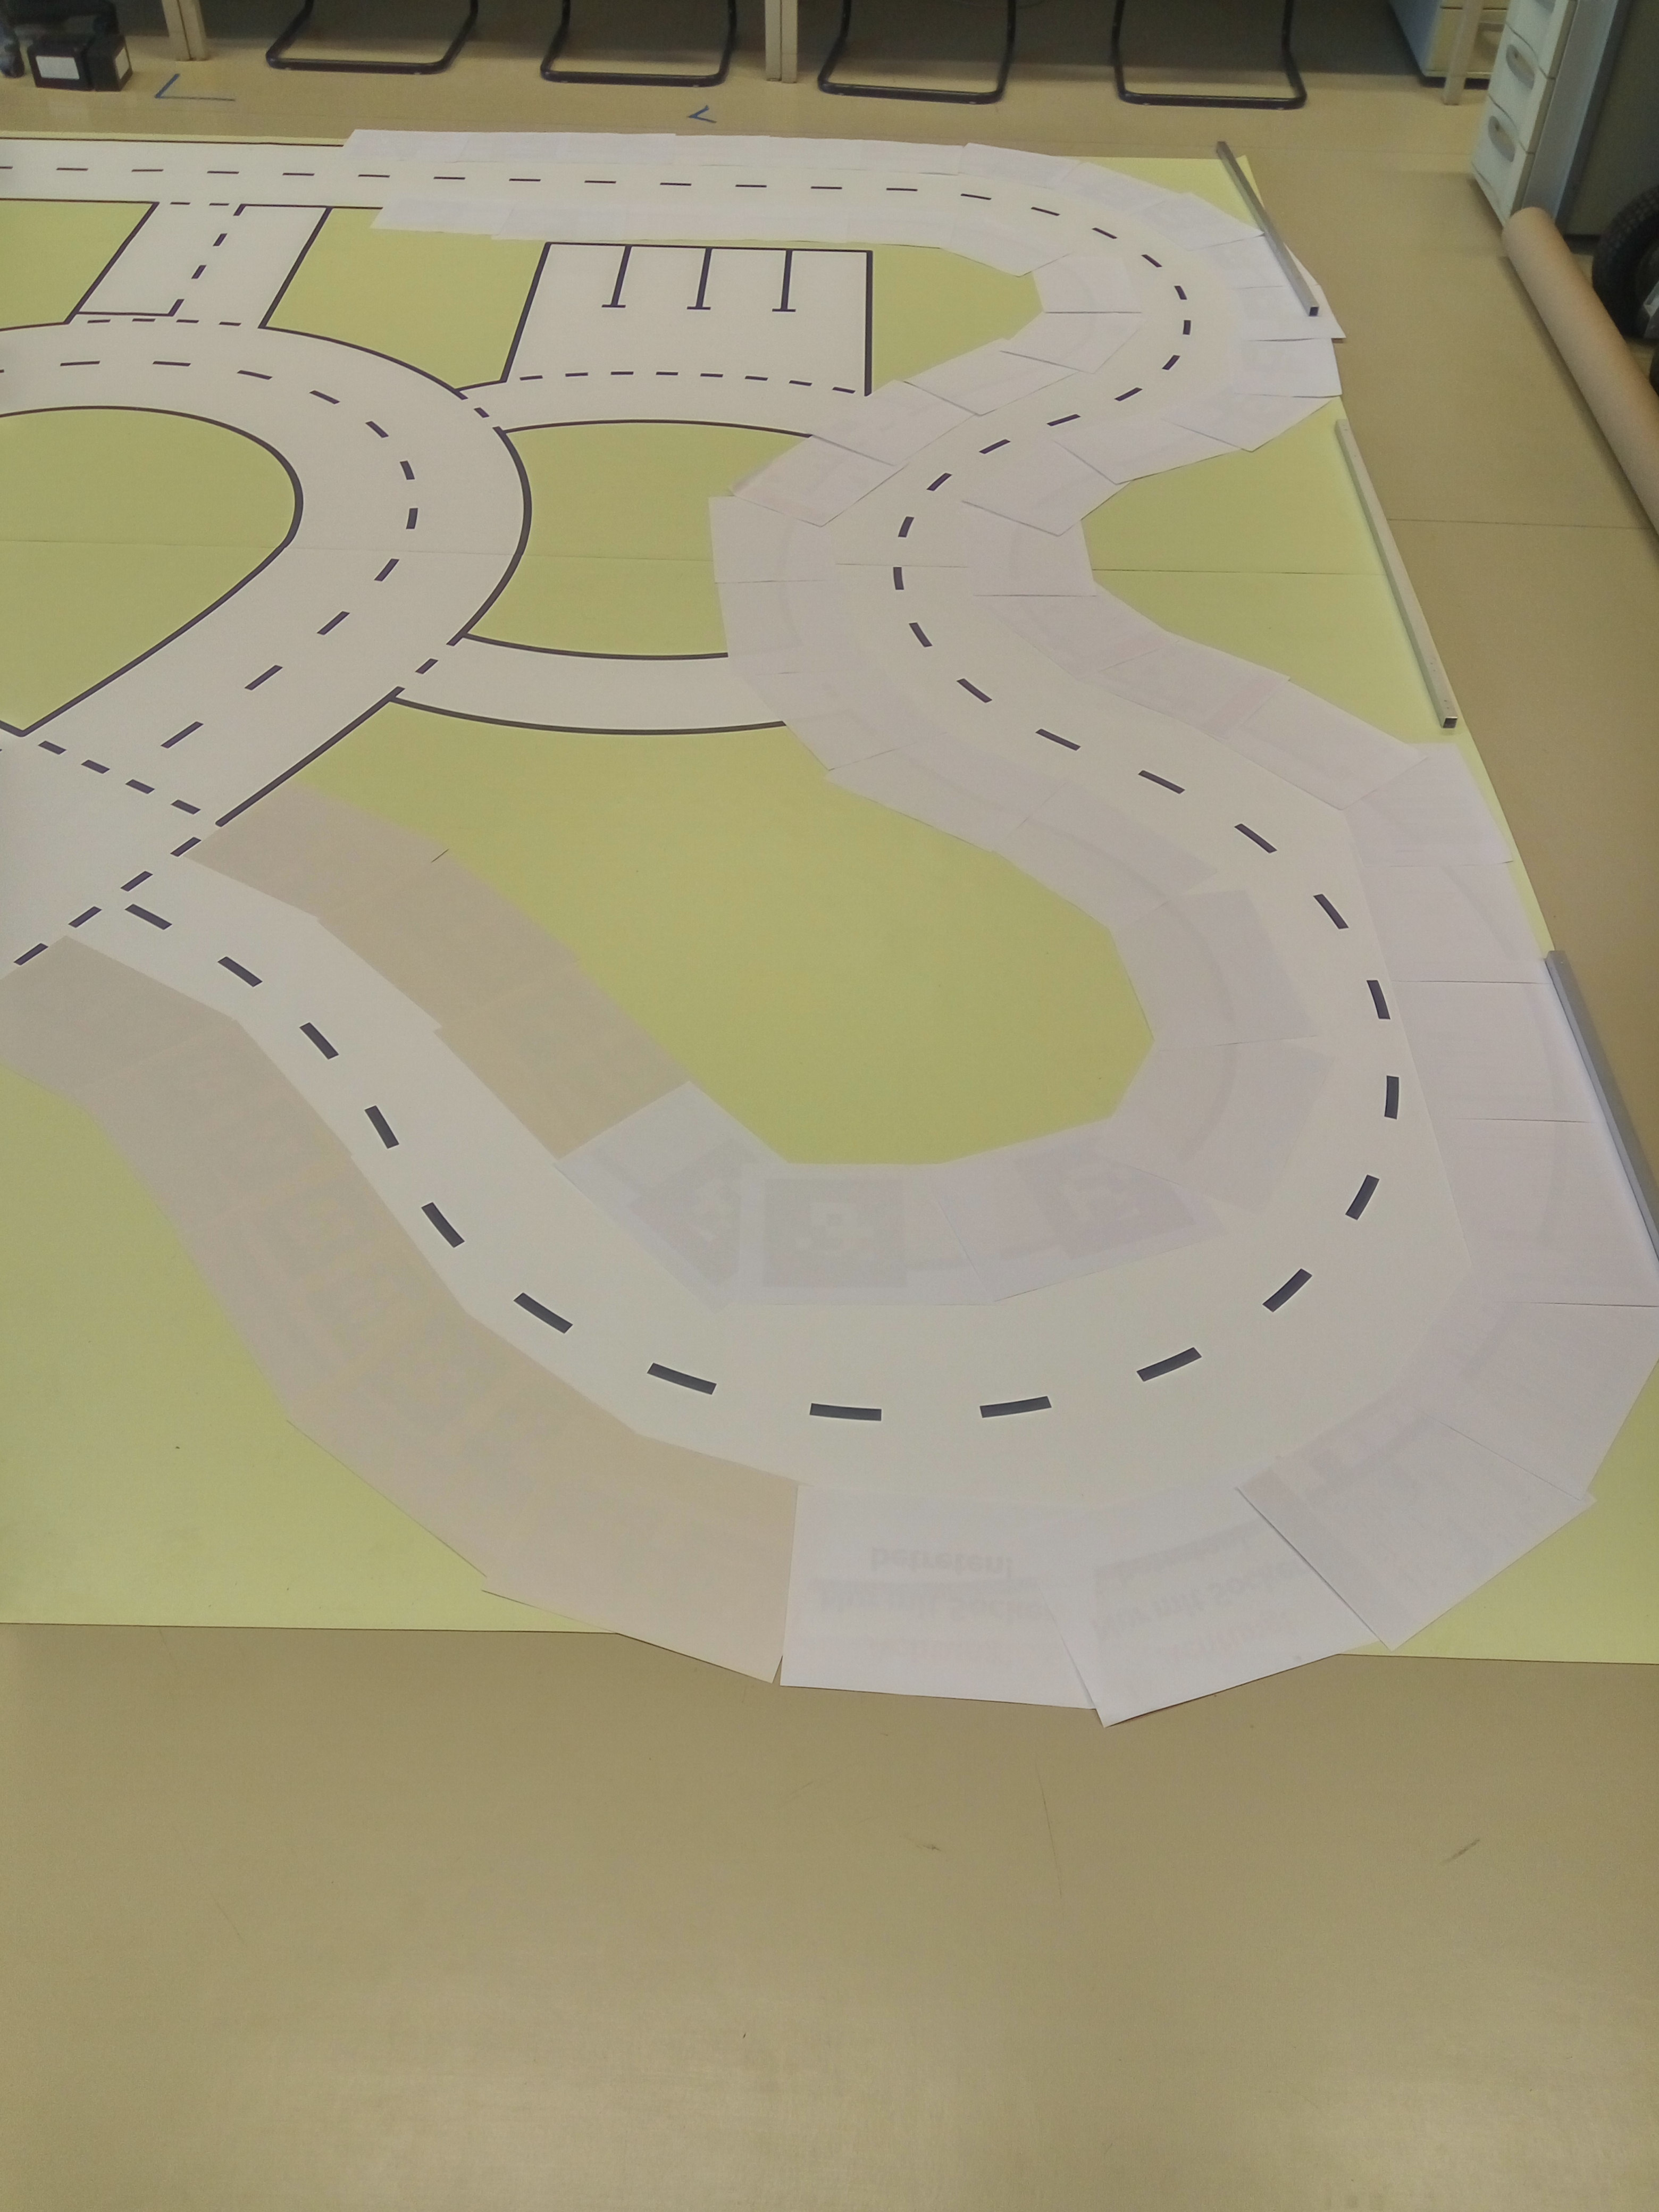
\includegraphics[height=0.35\textheight]{evaluation_riverflow_ohne_randlinie_versuchsaufbau.jpg}}
	\hfill
	\subfloat[Weltkarte ohne Randlinien \label{fig:evaluation:riverflow:ohneRandlinie:Weltkarte}]{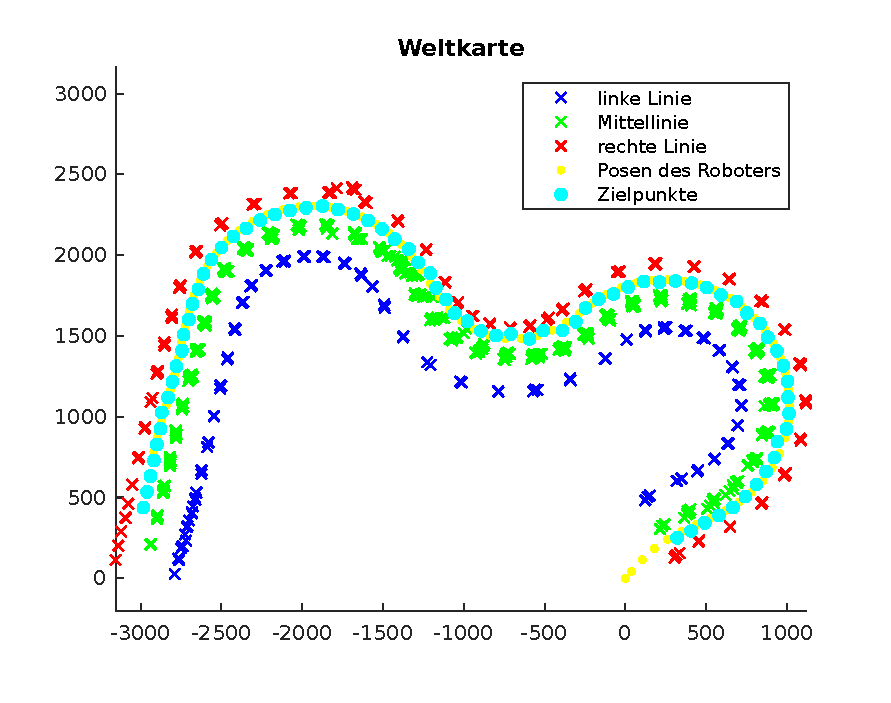
\includegraphics[height=0.35\textheight]{evaluation_riverflow_ohne_randlinie_worldmap.pdf}}
	\caption{Testfahrt mit durch weißes Papier abgedeckte Randlinien}
	\label{fig:evaluation:riverflow:ohneRandlinie}
\end{figure}

Im Plot~\ref{fig:evaluation:riverflow:ohneRandlinie:Weltkarte} fällt auf, dass trotz Abdeckung scheinbar einige Randlinienpunkte erkannt wurden. Mithilfe des in Abbildung~\ref{fig:evaluation:riverflow:ohneMittellinie:bspPlot} dargestellten Beispielplots lässt sich die Erklärung finden.

\begin{figure}[htbp] % [htb]
	\centering
	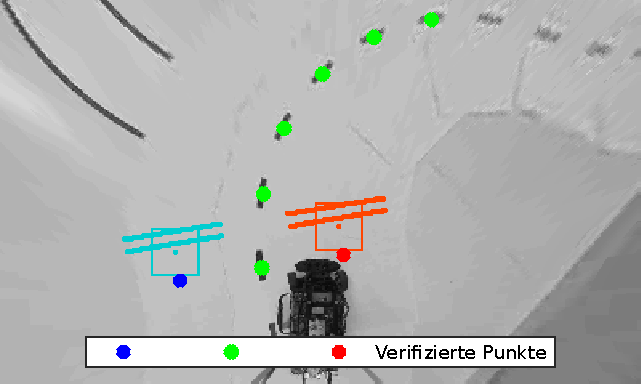
\includegraphics[width=0.7\textwidth]{evaluation_riverflow_ohne_randlinie_beispielplot.pdf}
	\caption{Punkterkennung bei abgedeckten Randlinien}
	\label{fig:evaluation:riverflow:ohneMittellinie:bspPlot}
\end{figure}

Ausgehend von der ersten mittleren Fahrbahnmarkierung werden die Startpunkte für die Randlinienerkennung bestimmt. Trotz fehlender Randlinienpunkte wurden die Startpunkte verifiziert und in die Karte aufgenommen. Da sie jedoch einzig den um die Fahrspurbreite verschobenen Mittellinienpunkt abbilden, stellen sie keinen informativen Mehrwert dar.

\subsection{Schlussfolgerungen}

Wir haben demonstriert, dass die Rand-und Mittellinienerkennung einzeln funktioniert und sich gegenseitig absichert. Das \gls{glos:tucar} ist nicht auf permanentes Vorhandensein von Mittel-/Randlinien oder deren fehlerfreie Erkennung angewiesen.
Die Zielpunktbestimmung als Voraussetzung für die Regelung ist somit gewährleistet, wenn mindestens die Mittellinie oder beide Randlinien erkannt wurden. Diese Sicherheit ist durch die Schwächen der jeweiligen Verfahren sinnvoll und notwendig. 

An der großen Kreuzung existiert beispielsweise keine mittlere Fahrbahnmarkierung, was die Randlinienerkennung notwendig macht. Gleichzeitig besitzt der Riverflow-Algorithmus den Nachteil, an ausreichend großen Lücken im Markierungsverlauf abzubrechen. Dieser Fall ist demonstrativ in Abbildung~\ref{fig:evaluation:riverflow:Randlinie:unterbrochen:bsp} dargestellt. 

\begin{figure}[htbp] % [htb]
	%\centering
	%\hfill
	\subfloat[Beispielbild einer Unterbrechung \label{fig:evaluation:riverflow:Randlinie:unterbrochen:bsp}]{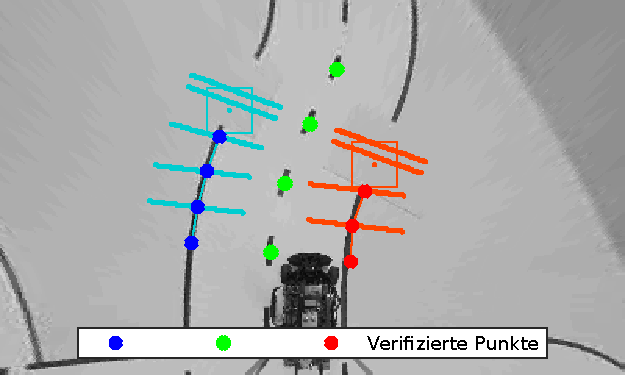
\includegraphics[height=0.25\textheight]{evaluation_riverflow_randlinie_unterbrochen_beispiel.pdf}}
	\hfill
	\subfloat[Länge der erkannten Linien \label{fig:evaluation:riverflow:Randlinie:unterbrochen:linienlaenge}]{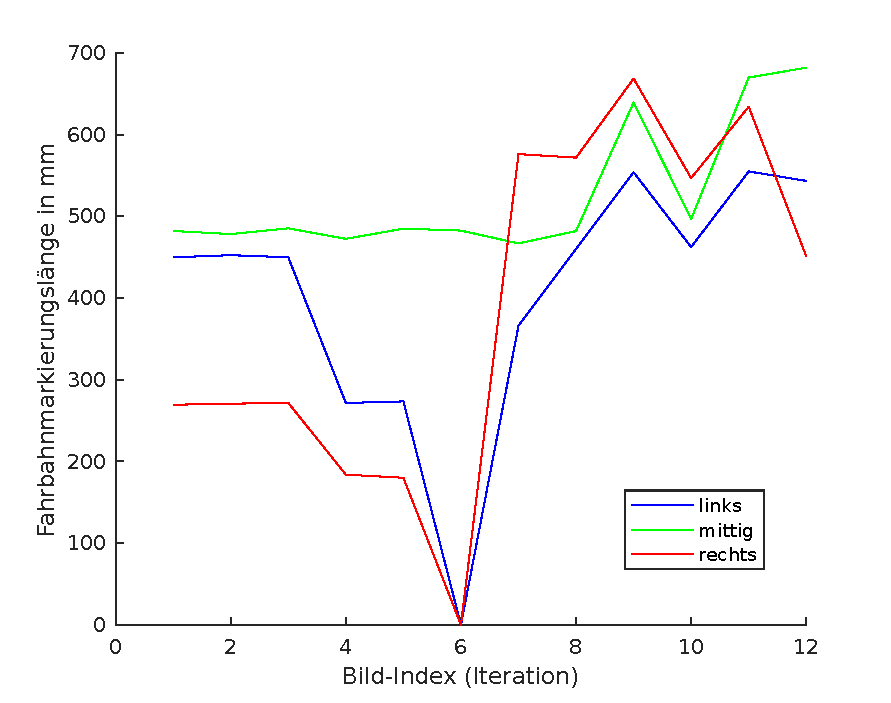
\includegraphics[height=0.25\textheight]{evaluation_riverflow_randlinie_unterbrochen_plot_linienlaenge.pdf}}
	\caption{Demonstration der Schwäche des Riverflow bei größeren Unterbrechungen in der Randlinie}
	\label{fig:evaluation:riverflow:Randlinie:unterbrochen}
\end{figure}

Die durch ein A4-Blatt unterbrochene Randlinie wird im folgenden Verlauf nicht länger erkannt. Dass die Linie in den vorherigen Bilditerationen ebenfalls nur bis zu jener Unterbrechung detektiert wurde, zeigt der Plot in Abbildung \ref{fig:evaluation:riverflow:Randlinie:unterbrochen:linienlaenge} durch die mit jedem Bildindex abnehmende Linienlänge. Die Fähigkeit, mittels Randlinienerkennung vorauszuschauen, ist somit bis zum Passieren dieser Unregelmäßigkeit nicht gegeben. Durch die möglich fehlerhafte Erkennung eines Mittellinienpunktes werden überdies ebenfalls alle nachfolgenden Mittellinienpunkte ignoriert, da auch hier die Verifikation des nächsten Punktes von der des aktuellen abhängt. 